\documentclass[UTF8]{ctexart}

\usepackage{amsmath, amssymb, amsthm}
\usepackage{mathrsfs}
\usepackage{graphicx}
\usepackage{float}
\usepackage{tikz}

% 图按章编号，并显示为“图 6-1”格式。
\numberwithin{figure}{section}
\renewcommand{\thefigure}{\thesection-\arabic{figure}}
\usepackage{tikz-cd}
\usepackage{pgfplots}
\usepackage{xltabular}
\usepackage{booktabs}
\usepackage{geometry}
\usepackage{extarrows}
\geometry{a4paper, margin=2cm}
\pgfplotsset{compat=1.18}
\usetikzlibrary{shapes.geometric, positioning, calc, decorations.pathreplacing, 3d}

\usepackage[numbers,square]{natbib}
\newcommand{\scite}[1]{\textsuperscript{\cite{#1}}}

\newtheorem{theorem}{定理}[subsection]
\newtheorem{proposition}[theorem]{命题}
\newtheorem{corollary}[theorem]{推论}
\newtheorem{lemma}[theorem]{引理}
\theoremstyle{definition}
\newtheorem{definition}[theorem]{定义}
\newtheoremstyle{examplestyle}{3pt}{3pt}{\itshape}{0pt}{\bfseries}{.}{.5em}{\thmnumber{例 \arabic{example}}\thmnote{\ (#3)}}
\theoremstyle{examplestyle}
\newtheorem{example}{}[subsection]
\theoremstyle{remark}
\newtheorem*{remark}{注}

\title{增广拉格朗日惩罚参数$c$的数值敏感性研究}
\author{}
\date{}

\usepackage[hidelinks]{hyperref}

\begin{document}

\maketitle

\section{研究背景与核心研究问题}
\label{sec:intro}

\subsection{增广拉格朗日方法}
\label{sec:alm-background}

增广拉格朗日方法（Augmented Lagrangian Method, ALM）是求解等式约束优化问题的经典框架\scite{bertsekas1982}。考虑如下等式约束优化问题
\begin{equation}
\label{eq:constrained}
\min_{x\in\mathbb{R}^n}\ f(x) \qquad \text{s.t.} \quad Ax=b,
\end{equation}
其中 $f:\mathbb{R}^n\to\mathbb{R}$ 为目标函数，$A\in\mathbb{R}^{m\times n}$ 为约束矩阵，$b\in\mathbb{R}^m$ 为约束右端项。ALM 在拉格朗日函数的基础上引入二次惩罚项，构造增广拉格朗日函数
\begin{equation}
\label{eq:alm}
\mathcal{L}_c(x,\lambda)=f(x)+\lambda^\top(Ax-b)+\frac{c}{2}\|Ax-b\|_2^2,
\end{equation}
其中 $c>0$ 为惩罚参数，$\lambda\in\mathbb{R}^m$ 为拉格朗日乘子。ALM 的每次外层迭代先对 $x$ 极小化 $\mathcal{L}_c(x,\lambda_k)$ 得到 $x_{k+1}$，再按乘子更新规则
\begin{equation}
\label{eq:multiplier-update}
\lambda_{k+1}=\lambda_k+c(Ax_{k+1}-b)
\end{equation}
更新乘子。该方法兼具拉格朗日法的对偶上升思想与罚函数法的强凸性，在凸优化、约束优化和分布式优化等领域有广泛应用。

\subsection{惩罚参数 $c$ 的关键作用}
\label{sec:c-role}

在增广拉格朗日函数 \eqref{eq:alm} 中，惩罚参数 $c$ 是调控约束惩罚强度的核心超参数，其取值直接影响算法的外层收敛速度与子问题求解难度：

\begin{itemize}
\item 当 $c$ 较小时，约束惩罚较弱，乘子更新对约束违反的修正力度有限，外层收敛通常较慢；
\item 当 $c$ 较大时，约束惩罚增强，外层收敛往往加快，但子问题海森矩阵 $H_c=H+cA^\top A$ 的条件数随之增大，内层求解难度与单轮计算成本上升。
\end{itemize}

因此，$c$ 的选取本质上是在外层迭代步数与内层求解成本之间进行权衡，理解这一权衡关系对 ALM 的高效实现和参数自适应具有重要意义。

\subsection{现有研究的不足}
\label{sec:gap}

现有研究多基于经验定性描述 $c$ 的权衡效应，但仍存在以下不足：

\begin{itemize}
\item 对“精确求解子问题”与“不精确求解子问题”两种场景下的行为差异缺乏系统区分，容易将不精确求解带来的数值现象错误归因于 ALM 本身；
\item 对最优惩罚参数与内层求解精度、原问题病态性的耦合关系缺少定量验证；
\item 对计算意义上的最优惩罚参数 $c^*$ 如何随问题条件数 $\kappa(H)$ 与内层精度 $\epsilon_{\mathrm{inner}}$ 漂移，尚未形成系统的实验结论。
\end{itemize}

这些不足使得实际使用中惩罚参数 $c$ 的选取往往依赖人工试错，缺乏可量化的指导准则。

\subsection{核心研究问题}
\label{sec:rqs}

针对上述不足，本实验以对称正定二次规划为基准测试问题，系统控制惩罚参数、内层求解精度、原问题条件数三类变量，围绕以下三个核心研究问题（Research Question, RQ）展开：

\begin{enumerate}
\item \textbf{RQ1：惩罚参数 $c$ 如何影响 ALM 的外层收敛行为？}
聚焦 $c$ 对原始残差 $\|Ax_k-b\|_2$ 与目标函数误差 $f(x_k)-f^*$ 演化规律的影响，并区分精确子问题求解与不精确子问题求解两种场景下的差异。
\item \textbf{RQ2：惩罚参数 $c$ 如何影响算法的整体计算效率？}
结合外层迭代开销与内层求解开销，量化二者的权衡关系，定位计算意义上的最优惩罚参数。
\item \textbf{RQ3：惩罚参数的最优取值是否依赖于问题条件数与内层求解精度？}
检验 $c^*=c^*(\kappa(H),\,\epsilon_{\mathrm{inner}})$ 的猜想，即最优惩罚参数是否同时由原问题条件数和内层求解精度决定，这是本实验最具创新性的核心内容。
\end{enumerate}



\section{理论基础与研究假设}
\label{sec:theory}

本章围绕惩罚参数 $c$ 的作用机制，给出精确 ALM 与不精确 ALM 的性质区分、子问题条件数的理论分析、内层迭代计算代价理论，并提出可检验的研究假设。

\subsection{两类 ALM 的性质区分}
\label{sec:alm-types}

本实验将 ALM 区分为两个层次：

\begin{enumerate}
\item \textbf{精确 ALM}：子问题求解到极高精度，近似理论意义上的全局最小化。在凸问题假设下，外层迭代具有严格收敛保证，目标函数与残差不会出现结构性震荡，$c$ 仅影响外层收敛速率。
\item \textbf{不精确 ALM}：子问题仅求解到有限精度（固定迭代步数或固定容差）。此时大 $c$ 会放大内层求解误差、加剧数值条件恶化，进而导致目标值波动、收敛平台抬高，甚至计算效率下降。
\end{enumerate}

震荡、平台等现象本质上来源于子问题不精确求解、数值条件恶化、浮点误差、终止准则不合理等实际因素，而非 ALM 本身的理论性质。

\subsection{子问题条件数的理论分析}
\label{sec:condition}

对于二次规划基准问题，子问题的海森矩阵为
\begin{equation}
\label{eq:Hc}
H_c=H+cA^\top A.
\end{equation}
若 $H\succ 0$ 且 $A$ 行满秩，则有以下性质：

\begin{itemize}
\item 最大特征值 $\lambda_{\max}(H_c)$ 随 $c$ 增大单调递增，当 $c\to\infty$ 时近似随 $c$ 线性增长；
\item 最小特征值 $\lambda_{\min}(H_c)\ge\lambda_{\min}(H)>0$，存在严格正下界；
\item 条件数 $\kappa(H_c)=\lambda_{\max}(H_c)/\lambda_{\min}(H_c)$ 的变化取决于 $H$ 与 $A^\top A$ 的谱结构：由于 $A^\top A\succeq0$，增大 $c$ 会使 $\lambda_{\max}(H_c)$ 与 $\lambda_{\min}(H_c)$ 均单调不减，但二者增长速率一般不同，因此 $\kappa(H_c)$ 并不必然单调上升；在本实验的大 $c$ 区域，$\kappa(H_c)$ 整体呈上升趋势。
\end{itemize}

该分析说明：增大 $c$ 在加强约束惩罚的同时，会改变子问题的谱结构，通常（但并非必然）恶化数值条件，从而增加内层求解难度。实际变化需结合 $H$ 与 $A^\top A$ 的谱方向综合判断。

\subsection{内层迭代的计算代价理论}
\label{sec:cg-cost}

采用共轭梯度法（CG）求解子问题线性系统时，经典收敛理论给出达到精度 $\epsilon_{\mathrm{inner}}$ 所需迭代步数的上界\scite{hestenes1952}：
\begin{equation}
\label{eq:cg-bound}
N_{\mathrm{CG}}\lesssim O\left(\sqrt{\kappa(H_c)}\cdot\log\frac{1}{\epsilon_{\mathrm{inner}}}\right),
\end{equation}
即内层迭代步数的上界与子问题条件数的平方根正相关，与求解精度的对数正相关。结合式 \eqref{eq:Hc} 的条件数性质，可以预期 $c$ 增大时单轮内层求解成本上升。

\subsection{正式研究假设}
\label{sec:hypotheses}

基于上述理论，提出以下可检验的研究假设：

\begin{enumerate}
\item \textbf{H1}：随着 $c$ 增大，外层迭代中原始残差的收敛速率总体提升；同时子问题条件数总体增大，单轮子问题的求解成本呈上升趋势，二者形成权衡关系。
\item \textbf{H2}：在不精确 ALM 场景下，总计算代价定义为总内层迭代数/运行时间，如果总成本曲线存在内部最小值，则称其表现为 U 型；若最优点落在扫描边界，则报告为边界最优。
\item \textbf{H3}：精确 ALM 场景下，外层收敛速度随 $c$ 增大单调提升，不会出现显著的 U 型效率拐点；震荡与收敛平台仅在不精确 ALM 的大 $c$ 区域出现。
\item \textbf{H4}：最优惩罚参数依赖于内层求解精度；随着内层求解精度变化，计算成本最优区域将发生系统性漂移。
\item \textbf{H5}：原问题条件数会影响惩罚参数的计算最优区域；随着问题病态性增强，大 $c$ 所带来的内层条件恶化效应预计更加显著。
\end{enumerate}

上述假设将指导后续实验设计与结果分析。

\section{测试问题构造}
\label{sec:test-problem}

\subsection{基准二次规划问题}
\label{sec:qp-benchmark}

选取对称正定二次规划作为核心测试问题，其优势在于子问题结构显式、条件数可精确计算、最优解可通过 KKT 系统精确求解：
\begin{equation}
\label{eq:qp}
\min_{x\in\mathbb{R}^n}\ \frac{1}{2}x^\top H x-q^\top x \qquad \text{s.t.} \quad Ax=b,
\end{equation}
其中 $H\succ 0$ 为对称正定矩阵，$q\in\mathbb{R}^n$，$A\in\mathbb{R}^{m\times n}$，$b\in\mathbb{R}^m$。基础参数设置如下：
\begin{itemize}
\item 问题规模：变量维数 $n=100$，约束个数 $m=20$；
\item $A$：随机稠密矩阵，保证行满秩；
\item $b$：通过预设最优解 $x^*$ 反算生成，确保可行且最优值、最优乘子已知，用于误差计算。
\end{itemize}

\subsection{多条件数测试集}
\label{sec:kappa-set}

构造 4 组不同条件数的 $H$ 矩阵，作为独立实验因素：
\begin{equation}
\label{eq:kappa-grid}
\kappa(H)\in\{10^1,\,10^2,\,10^3,\,10^4\},
\end{equation}
用于研究原问题病态性与惩罚参数 $c$ 的耦合效应。


\section{实验变量与控制规范}
\label{sec:control}

\begin{remark}
本章为实验变量与控制规范说明，用于保证实验可重复性，不涉及理论推导与算法实现代码；若报告聚焦理论与算法主线，可将本章作为可选内容酌情精简或忽略。
\end{remark}

\subsection{核心实验因素}
\label{sec:factors}

\begin{enumerate}
\item \textbf{惩罚参数 $c$}：对数等间距选取 9 个值，覆盖 9 个数量级
\[
c\in\{10^{-4},10^{-3},10^{-2},10^{-1},10^{0},10^{1},10^{2},10^{3},10^{4}\}.
\]
\item \textbf{内层求解精度 $\epsilon_{\mathrm{inner}}$}：选取 3 个典型精度等级，额外设置高精度组作为精确 ALM 近似
\[
\epsilon_{\mathrm{inner}}\in\{10^{-2},10^{-4},10^{-6},10^{-12}\}.
\]
\item \textbf{原问题条件数 $\kappa(H)$}：4 个梯度等级
\[
\kappa(H)\in\{10^1,10^2,10^3,10^4\}.
\]
\end{enumerate}

\subsection{统一控制变量}
\label{sec:controls}

为保证单一变量原则，所有实验组采用一致的基础设置：
\begin{itemize}
\item 初始点：$x_0=\boldsymbol{0}$；
\item 初始乘子：$\lambda_0=\boldsymbol{0}$；
\item 外层终止准则：原始残差 $\|r_p\|_2\le10^{-6}$ 且平稳性残差 $\|r_s\|_2\le10^{-6}$，或最大外层迭代 500 步；
\item 乘子更新规则：$\lambda_{k+1}=\lambda_k+c(Ax_{k+1}-b)$；
\item 每组参数设置重复 3 次随机实验，取平均值作为统计结果。
\end{itemize}

\subsection{残差术语规范}
\label{sec:residuals}

统一采用 ALM 标准残差定义，不使用 ADMM 语境下的“对偶残差”表述：
\begin{enumerate}
\item \textbf{原始残差（primal residual）}：$r_p^k=Ax_k-b$，衡量约束违反程度；
\item \textbf{平稳性残差（stationarity residual）}：$r_s^k=\nabla f(x_k)+A^\top\lambda_k$，衡量一阶平稳性条件满足程度。
\end{enumerate}

\section{核心实验设计}
\label{sec:experiments}

\subsection{实验 1：基础 $c$-敏感性分析}
\label{sec:exp1}

\textbf{实验定位：}基础基准实验，回答 RQ1 的外层收敛规律。

\textbf{固定条件：}基准问题 $\kappa(H)=100$，内层精度设置两组对照（精确组 $\epsilon_{\mathrm{inner}}=10^{-12}$、典型不精确组 $\epsilon_{\mathrm{inner}}=10^{-4}$）。

\textbf{扫描变量：}惩罚参数 $c\in\{10^{-4},10^{-3},\dots,10^{4}\}$。

\textbf{核心观测指标：}
\begin{itemize}
\item 逐轮原始残差 $r_p(k)$ 演化；
\item 逐轮平稳性残差 $r_s(k)$ 演化；
\item 收敛所需外层迭代次数 $N_{\mathrm{outer}}$。
\end{itemize}

\textbf{实验内容与分析要点：}
\begin{enumerate}
\item 分别在精确 ALM 与不精确 ALM 两种场景下，遍历所有 $c$ 值运行算法，记录完整收敛轨迹；
\item 绘制不同 $c$ 下的残差收敛曲线（对数坐标），对比外层收敛速率随 $c$ 的变化趋势；
\item 对比精确与不精确场景的差异：验证精确场景下收敛速度随 $c$ 单调提升，无结构性震荡；不精确场景下大 $c$ 区域出现收敛平台与波动；
\item 验证假设 H1 与 H3 的外层收敛部分。
\end{enumerate}

\subsection{实验 2：计算成本权衡与最优 $c$}
\label{sec:exp2}

\textbf{实验定位：}效率分析实验，回答 RQ2 的计算权衡问题。

\textbf{固定条件：}基准问题 $\kappa(H)=100$，典型不精确场景 $\epsilon_{\mathrm{inner}}=10^{-4}$。

\textbf{扫描变量：}惩罚参数 $c$ 全网格。

\textbf{核心观测指标：}
\begin{itemize}
\item 单轮平均内层迭代数 $N_{\mathrm{inner}}$；
\item 收敛所需外层迭代数 $N_{\mathrm{outer}}$；
\item 全程累计总内层迭代数 $N_{\mathrm{inner,total}}$；
\item 总 CPU 运行时间。
\end{itemize}

\textbf{实验内容与分析要点：}
\begin{enumerate}
\item 统计每个 $c$ 对应的外层迭代开销、内层单轮开销、总计算开销；
\item 绘制“总内层迭代数 vs $c$”与“CPU 时间 vs $c$”曲线，验证是否呈现先降后升的 U 型分布；
\item 定位计算意义上的最优惩罚参数 $c^*_{\mathrm{computational}}$，即总计算代价最小的 $c$ 取值；
\item 分解 U 型曲线的成因：左侧由外层收敛过慢主导，右侧由内层条件数恶化主导，验证假设 H2。
\end{enumerate}

\subsection{实验 3：条件数 $\times$ 内层精度的耦合影响}
\label{sec:exp3}

\textbf{实验定位：}核心创新实验，回答 RQ3 的最优参数依赖性问题。

\textbf{改变变量：}原问题条件数 $\kappa(H)\in\{10^1,10^2,10^3,10^4\}$、内层求解精度 $\epsilon_{\mathrm{inner}}\in\{10^{-2},10^{-4},10^{-6}\}$；额外纳入 $\epsilon_{\mathrm{inner}}=10^{-12}$ 作为 high-accuracy reference，用于近似精确 ALM。

\textbf{扫描变量：}每组参数组合下遍历全量 $c$。

\textbf{核心问题：}最优惩罚参数是否同时依赖于问题条件数与内层精度，即 $c^*=c^*(\kappa(H),\,\epsilon_{\mathrm{inner}})$？

\textbf{实验内容与分析要点：}
\begin{enumerate}
\item 对 $4\times3$ 组参数组合，分别重复实验 2 的完整流程，计算每组对应的最优 $c^*$；
\item 固定内层精度，对比不同条件数下 $c^*$ 的变化：验证原问题越病态，最优 $c^*$ 越小（假设 H5）；
\item 固定问题条件数，对比不同内层精度下 $c^*$ 的变化：验证内层精度越松，最优 $c^*$ 越小（假设 H4）；
\item 绘制二维热力图或多组对比曲线，例如横轴 $\log_{10}\kappa$、纵轴 $\log_{10}\epsilon_{\mathrm{inner}}$、颜色 $\log_{10}c^*$，系统展示 $c^*$ 随两个因素的漂移规律；如果有规律，尝试拟合
\[
\log c^*=a+b\log\kappa+d\log\epsilon_{\mathrm{inner}},
\]
如果拟合不出线性关系，则说明 $c^*$ 不满足简单幂律关系。
\end{enumerate}

\subsection{实验 4：固定 $c$ vs 自适应 $c$}
\label{sec:exp4}

\textbf{实验定位：}延伸应用实验，作为前三部分结论的自然落地。

\textbf{对比对象：}
\begin{itemize}
\item 对照组：实验 2 中得到的最优固定 $c_0=c^*_{\mathrm{computational}}$；
\item 实验组：两种经典自适应 $c$ 策略
\begin{enumerate}
\item 固定倍率递增：每 5 轮外层迭代，令 $c_{k+1}=1.5\cdot c_k$；
\item 残差平衡自适应：若原始残差 $>10$ 倍平稳性残差，则增大 $c$，否则保持不变；增大方式为倍增 $c_{k+1}=\gamma c_k$（$\gamma$ 取 2 或 5），同时设置 $c$ 的最大值和最小值。
\end{enumerate}
\end{itemize}

\textbf{核心问题：}自适应调整策略能否在无需预调参的前提下，逼近最优固定 $c$ 的计算效率？

\textbf{实验内容与分析要点：}
\begin{enumerate}
\item 在基准问题与多组条件数问题上，分别运行固定最优 $c$ 与自适应策略；
\item 对比总计算效率、收敛平稳性、最终精度三个维度的表现；
\item 验证自适应策略的价值：在问题特性未知时，能否自动找到接近最优的惩罚强度，避免手动调参成本。
\end{enumerate}

\section{观测指标体系汇总}
\label{sec:metrics}

本章汇总实验所需观测指标，分为收敛轨迹类、计算效率类和数值条件类三类。

\subsection{收敛轨迹类（逐轮记录）}
\label{sec:metrics-trajectory}

\begin{itemize}
\item 原始残差 $\|r_p^k\|_2$；
\item 目标函数相对误差 $|f(x_k)-f^*|/|f^*|$；
\item 平稳性残差 $\|r_s^k\|_2$；
\item 乘子相对误差 $\|\lambda_k-\lambda^*\|_2/\|\lambda^*\|_2$。
\end{itemize}

\subsection{计算效率类（聚合统计）}
\label{sec:metrics-efficiency}

\begin{itemize}
\item 收敛所需外层迭代次数；
\item 单轮平均内层迭代次数；
\item 全程累计总内层迭代次数；
\item 总 CPU 运行时间。
\end{itemize}

\subsection{数值条件类}
\label{sec:metrics-condition}

\begin{itemize}
\item 子问题海森矩阵条件数 $\kappa(H_c)$；
\item 子问题最大/最小特征值；
\item 内层迭代步数与条件数的相关系数。
\end{itemize}

\section{结果判定标准}
\label{sec:verdict}

各研究假设的成立判定以实验数据为准，具体判定规则明确如下：

\begin{enumerate}
\item \textbf{H1 成立判定}：随 $c$ 增大，达到相同原始残差精度所需的外层迭代数总体下降，即外层收敛速率总体提升；同时单轮平均内层迭代数总体上升。两个趋势同时出现时，认为 H1 成立，即 $c$ 在外层收敛速度与内层求解成本之间形成权衡关系。
\item \textbf{H2 成立判定}：在不精确 ALM 场景下，考察总计算代价（总内层迭代数或 CPU 时间）随 $c$ 的变化曲线。若曲线存在内部最小值，则表现为 U 型，H2 成立；若最优 $c$ 落在扫描边界，则报告为边界最优，并明确标注该边界情形。
\item \textbf{H3 成立判定}：在精确 ALM 场景下，外层收敛速度随 $c$ 增大单调提升（或达到相同残差精度所需的外层迭代数单调不增），且无显著震荡与收敛平台；同时，震荡与收敛平台仅在不精确 ALM 的大 $c$ 区域出现。若精确场景出现明显震荡或平台，则 H3 不成立。
\item \textbf{H4 成立判定}：固定问题条件数，随着内层求解精度变松（$\epsilon_{\mathrm{inner}}$ 增大），最优惩罚参数 $c^*$ 总体向更小方向漂移；若 $c^*$ 随 $\epsilon_{\mathrm{inner}}$ 出现系统性漂移且方向与假设一致，则 H4 成立。
\item \textbf{H5 成立判定}：固定内层精度，随着原问题条件数 $\kappa(H)$ 增大（问题更病态），最优惩罚参数 $c^*$ 总体向更小方向漂移，且大 $c$ 区域的内层条件恶化效应（如单轮内层迭代数、子问题条件数）增强更显著；若满足上述规律，则 H5 成立。
\end{enumerate}

\section{实验结果与分析}
\label{sec:results}

本章基于批量实验结果，依次回答三个核心研究问题，并对研究假设 H1--H5 的成立情况进行检验。所有统计均基于达到外层终止条件的收敛试验，最优惩罚参数 $c^*$ 定义为在收敛试验中平均总内层迭代次数最小的 $c$。

\subsection{实验 1：外层收敛行为与 RQ1}
\label{sec:res-exp1}

图~\ref{fig:conv} 给出了 $\kappa(H)=100$ 下不同惩罚参数 $c$ 的原始残差收敛轨迹，分别对应典型不精确内层求解（$\epsilon_{\mathrm{inner}}=10^{-4}$）与精确内层求解（$\epsilon_{\mathrm{inner}}=10^{-12}$）。

\begin{figure}[H]
\centering
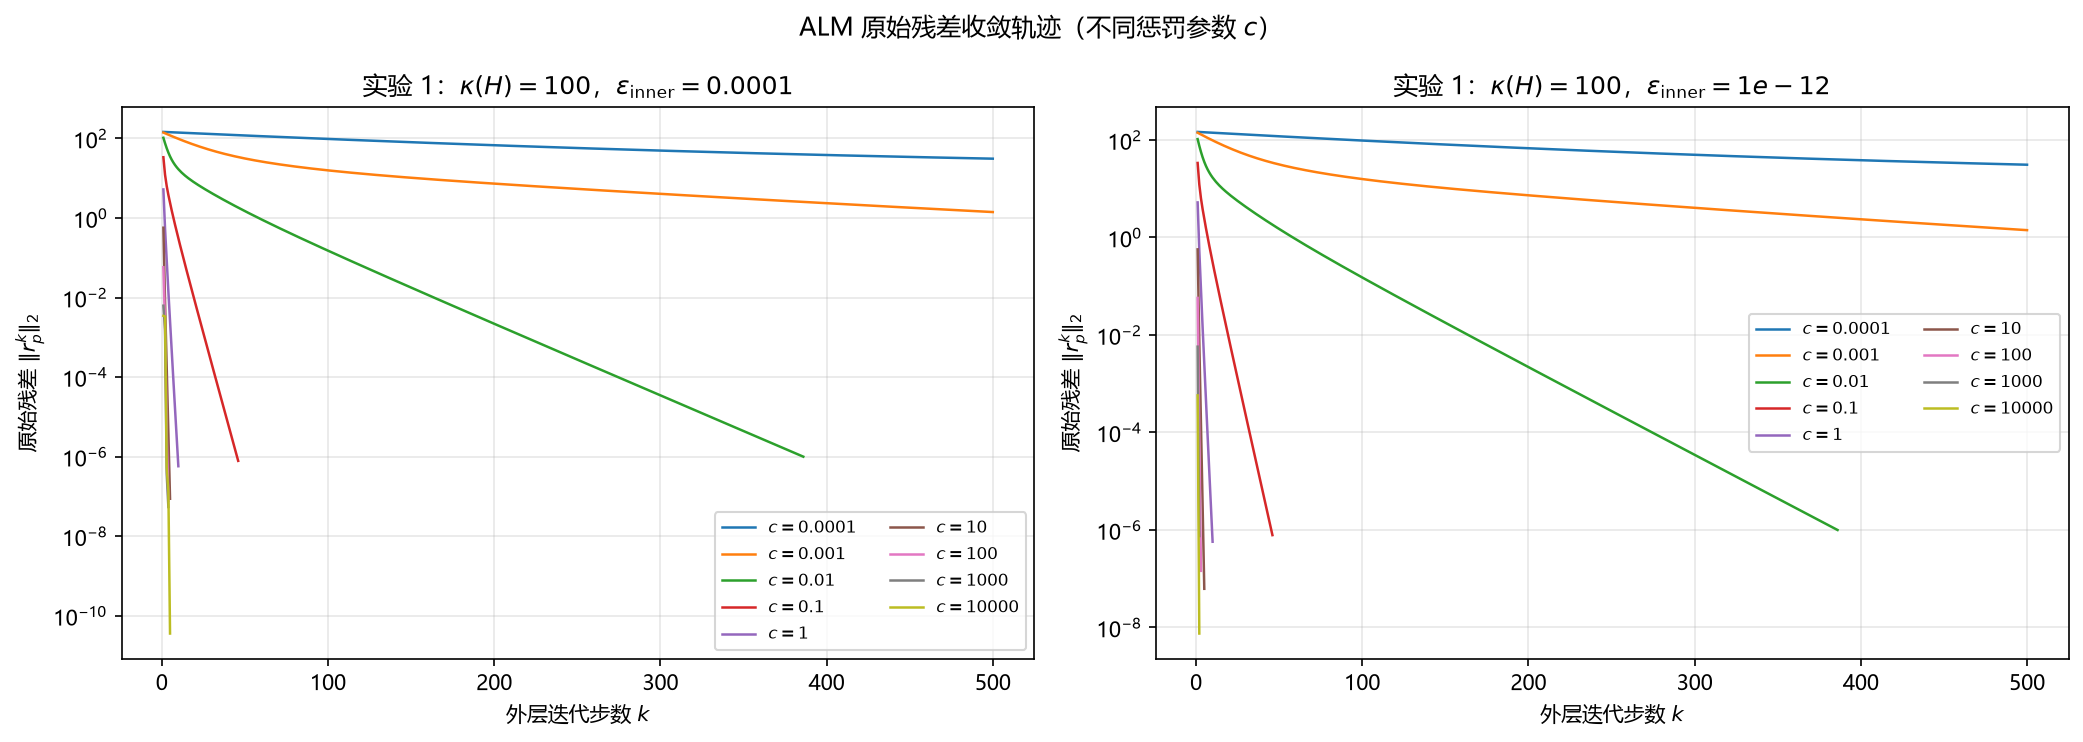
\includegraphics[width=0.98\textwidth]{figures/fig1_convergence.png}
\caption{实验 1：不同惩罚参数 $c$ 下 ALM 原始残差收敛轨迹}
\label{fig:conv}
\end{figure}

可以看出：
\begin{itemize}
\item 在可收敛的 $c$ 范围内，$c$ 越大，原始残差下降越快，外层所需迭代数越少，说明增大 $c$ 总体提升外层收敛速率；
\item 精确内层求解（右图）下，各 $c$ 的收敛轨迹平滑，未出现结构性震荡；
\item 不精确内层求解（左图）下，过小的 $c$ 收敛缓慢；较大的 $c$ 原始残差下降更快。需要说明的是，图~\ref{fig:conv} 仅展示原始残差轨迹，平稳性残差是否达到终止容差需结合批量统计判断：部分大 $c$ 组合的平稳性残差未能同步达到 $10^{-6}$，表现为不精确 ALM 的数值平台。
\end{itemize}

从图~\ref{fig:conv} 还可看到，左右两图的原始残差轨迹形态接近，说明内层精度对原始残差下降轨迹的影响有限；二者的差异主要体现在平稳性残差是否达到终止容差。因此，RQ1 的回答为：惩罚参数 $c$ 主要通过约束惩罚强度影响外层收敛速率；$c$ 越大，原始残差收敛越快，但该结论依赖于内层求解精度。在精确 ALM 下，$c$ 的作用主要体现在收敛速率；在不精确 ALM 下，过大的 $c$ 会因内层误差放大而产生收敛平台（需结合平稳性残差统计判断）。

\subsection{实验 2：计算效率权衡与 RQ2}
\label{sec:res-exp2}

图~\ref{fig:ustar} 给出 $\kappa(H)=100$、$\epsilon_{\mathrm{inner}}=10^{-4}$ 下平均总内层迭代次数随 $c$ 的变化。

\begin{figure}[H]
\centering
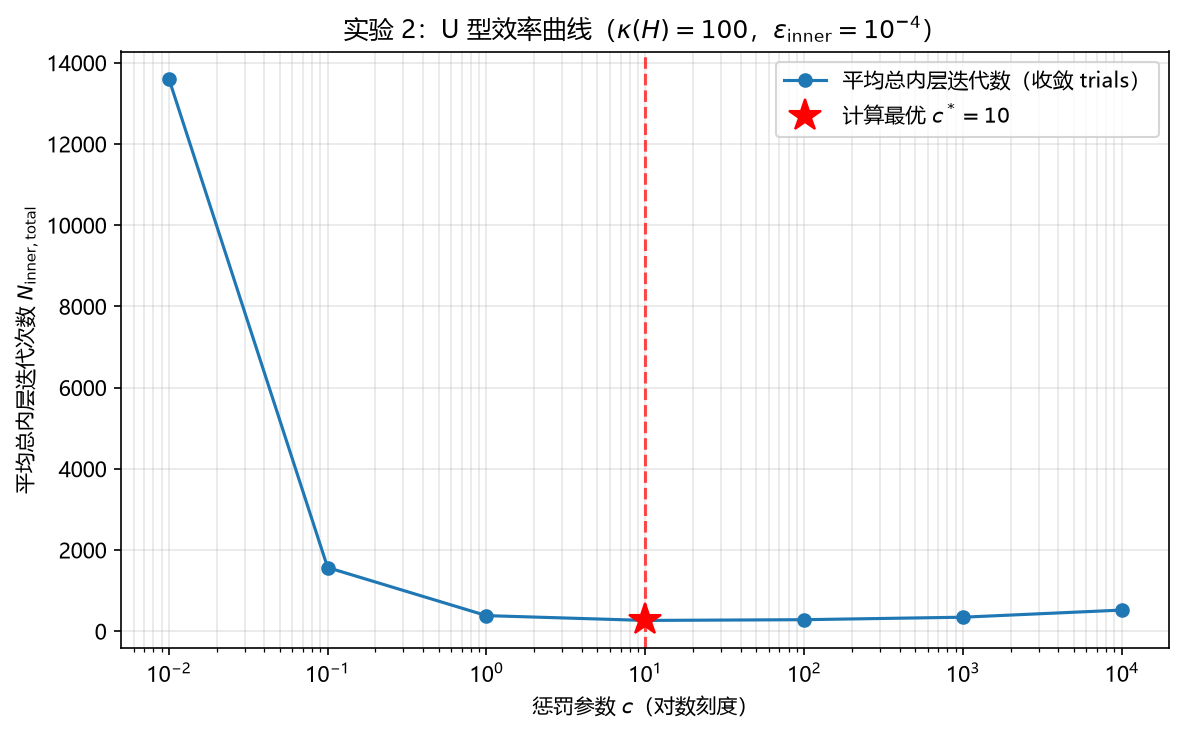
\includegraphics[width=0.8\textwidth]{figures/fig2_ustar.png}
\caption{实验 2：总内层迭代次数随惩罚参数 $c$ 的变化，呈现 U 型曲线}
\label{fig:ustar}
\end{figure}

结果显示：
\begin{itemize}
\item 总内层迭代次数随 $c$ 先降后升，呈明显 U 型；
\item 计算最优惩罚参数约为 $c^*=10$，此时平均总内层迭代次数约 266；
\item 左侧（小 $c$）成本高由外层收敛过慢主导，右侧（大 $c$）成本上升由子问题条件数恶化、单轮内层迭代增加主导。
\end{itemize}

因此，RQ2 的回答为：$c$ 对整体计算效率存在非单调影响，计算意义上存在最优惩罚参数 $c^*$，其取值由外层迭代数与内层求解成本的权衡决定。

\subsection{实验 3：最优惩罚参数的依赖规律与 RQ3}
\label{sec:res-exp3}

图~\ref{fig:eps-compare} 和图~\ref{fig:kappa-compare} 分别给出固定条件数下不同内层精度的 U 型曲线，以及固定内层精度下不同条件数的 U 型曲线。

\begin{figure}[H]
\centering
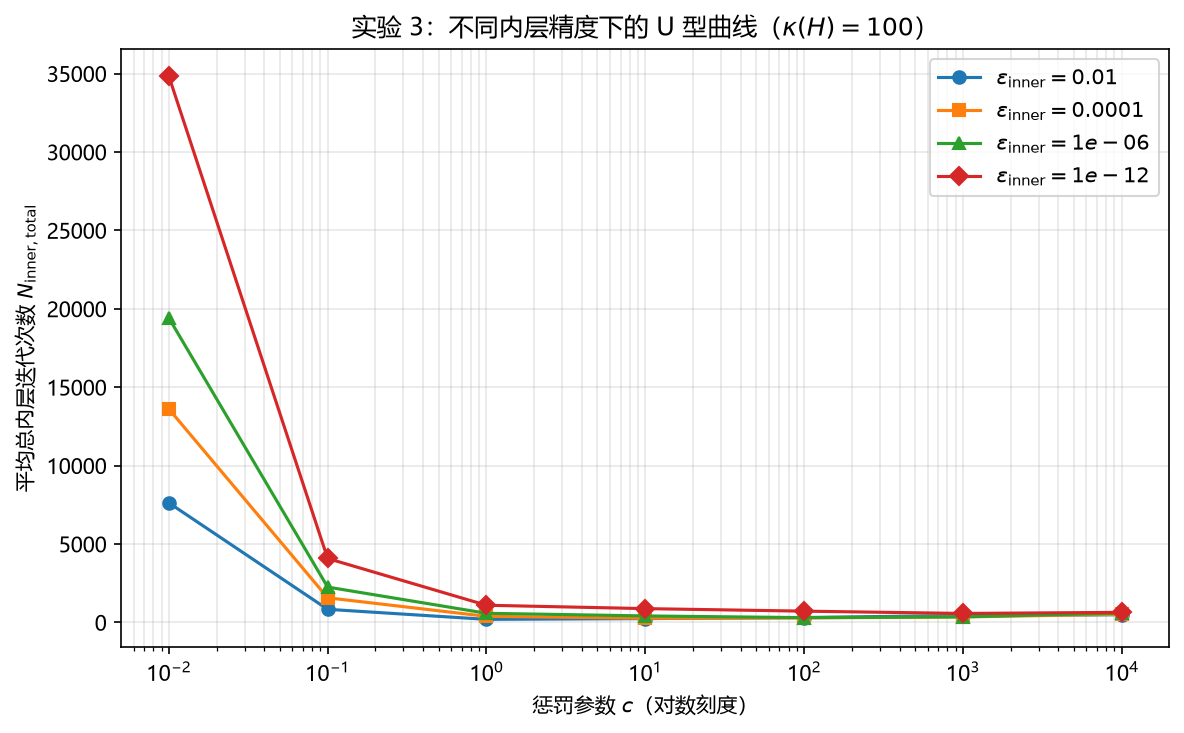
\includegraphics[width=0.8\textwidth]{figures/fig3_eps_compare.png}
\caption{实验 3：固定 $\kappa(H)=100$，不同内层精度下的 U 型曲线对比}
\label{fig:eps-compare}
\end{figure}

\begin{figure}[H]
\centering
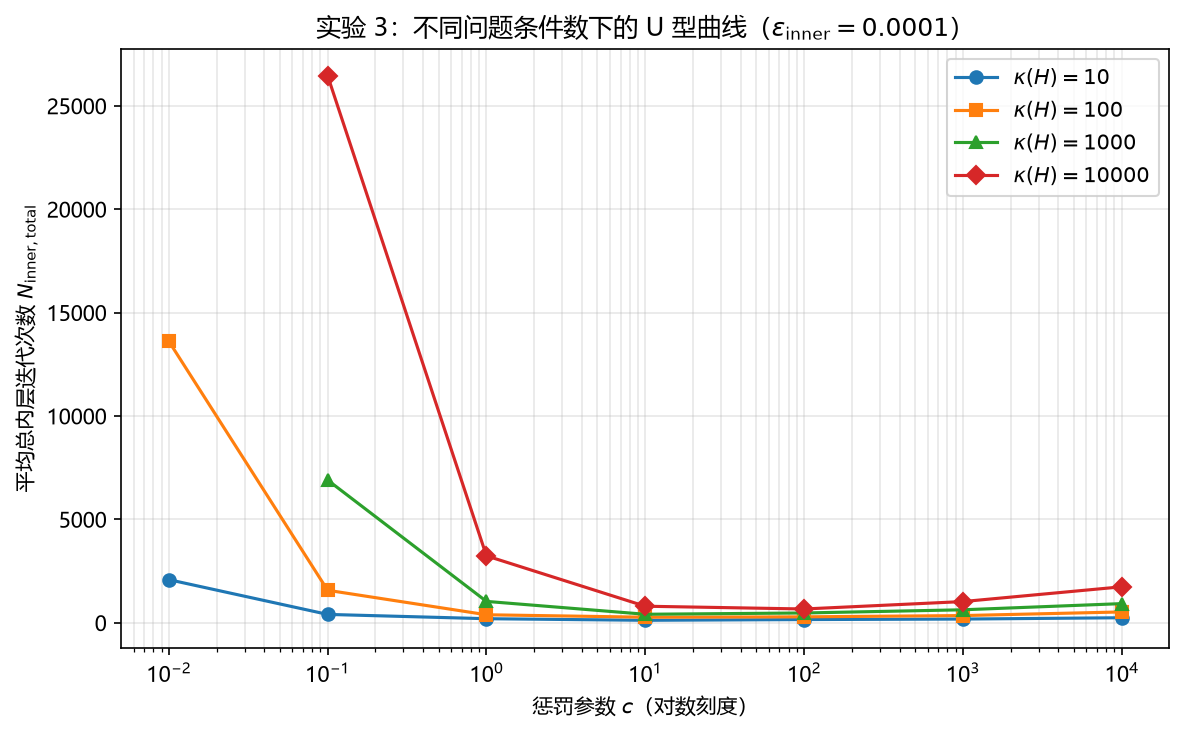
\includegraphics[width=0.8\textwidth]{figures/fig4_kappa_compare.png}
\caption{实验 3：固定 $\epsilon_{\mathrm{inner}}=10^{-4}$，不同条件数下的 U 型曲线对比}
\label{fig:kappa-compare}
\end{figure}

图~\ref{fig:cstar-heatmap} 给出 $c^*$ 随 $\kappa(H)$ 与 $\epsilon_{\mathrm{inner}}$ 漂移的二维热力图。

\begin{figure}[H]
\centering
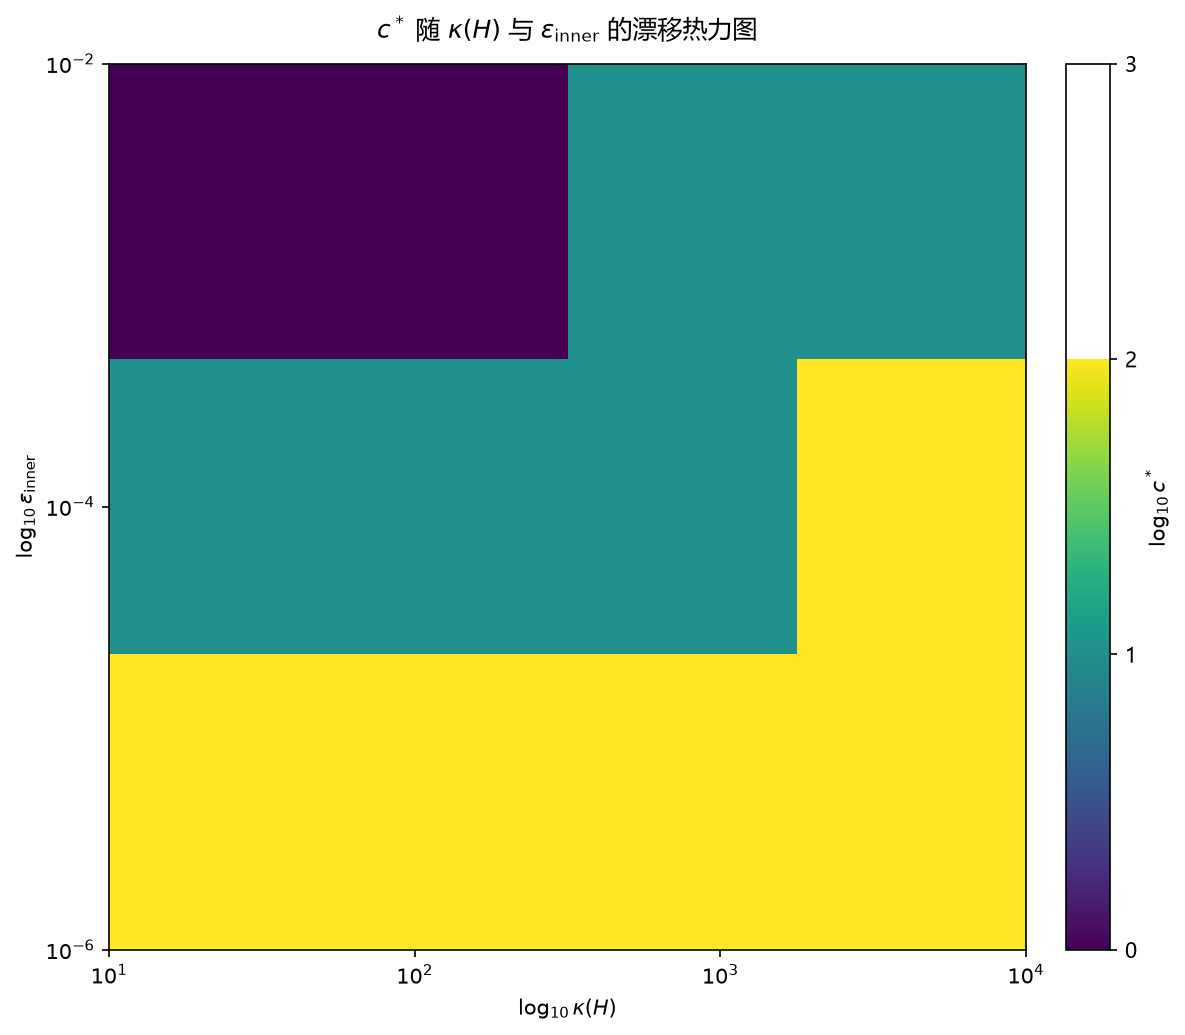
\includegraphics[width=0.72\textwidth]{figures/fig6_cstar_heatmap.png}
\caption{实验 3：$c^*$ 随 $\kappa(H)$ 与 $\epsilon_{\mathrm{inner}}$ 的漂移热力图}
\label{fig:cstar-heatmap}
\end{figure}

从图中可以观察到：
\begin{itemize}
\item 固定 $\kappa(H)$ 时，$c^*$ 随 $\epsilon_{\mathrm{inner}}$ 增大而明显减小。例如 $\kappa(H)=100$ 时，$\epsilon_{\mathrm{inner}}=10^{-12},10^{-6},10^{-4},10^{-2}$ 对应的 $c^*$ 分别约为 $1000,100,10,1$，支持假设 H4；
\item 固定 $\epsilon_{\mathrm{inner}}$ 时，$c^*$ 随 $\kappa(H)$ 的变化较弱，且方向为略微增大而非减小。例如 $\epsilon_{\mathrm{inner}}=10^{-2}$ 时，$\kappa(H)=10,100$ 对应 $c^*=1$，而 $\kappa(H)=1000,10000$ 对应 $c^*=10$。这与假设 H5 的预期方向相反，因此 H5 未得到支持；
\item 对 $4\times3$ 组参数进行幂律拟合得到
\[
\log_{10} c^* = -0.83 + 0.23\log_{10}\kappa(H) - 0.37\log_{10}\epsilon_{\mathrm{inner}}, \qquad R^2=0.851.
\]
该结果表明 $c^*$ 对内层精度的依赖明显（系数 $-0.37$），对条件数的依赖较弱且为正（系数 $0.23$），不满足原假设中“越病态 $c^*$ 越小”的简单幂律方向。
\end{itemize}

为了解释 H5 未支持的原因，图~\ref{fig:hc-condition} 给出了子问题条件数 $\kappa(H_c)$ 随惩罚参数 $c$ 的变化，并标注了各参数组合的计算最优 $c^*$。

\begin{figure}[H]
\centering
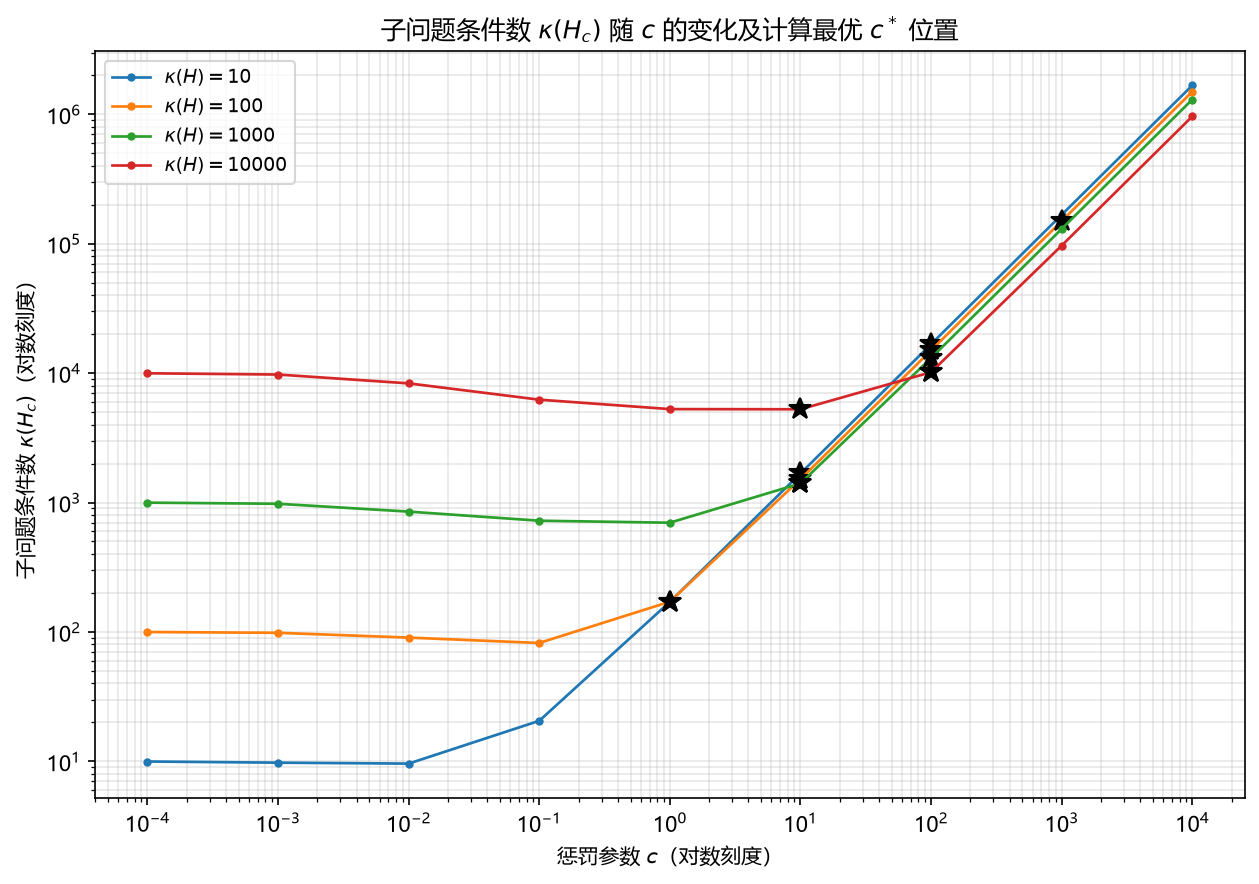
\includegraphics[width=0.85\textwidth]{figures/fig7_hc_condition.png}
\caption{子问题条件数 $\kappa(H_c)$ 随 $c$ 的变化及计算最优 $c^*$ 位置}
\label{fig:hc-condition}
\end{figure}

可以看出，$\kappa(H_c)$ 并非仅由 $\kappa(H)$ 决定，而是同时取决于 $c$、$A^\top A$ 以及二者谱结构的相互作用。例如，在 $\epsilon_{\mathrm{inner}}=10^{-2}$ 时，$\kappa(H)=10,100,1000,10000$ 对应的最优 $c^*$ 处 $\kappa(H_{c^*})$ 分别约为 $1.7\times10^2,1.7\times10^2,1.4\times10^3,5.3\times10^3$，并未随 $\kappa(H)$ 等比例恶化。此外，图~\ref{fig:hc-condition} 还显示，当 $c$ 较大时，不同 $\kappa(H)$ 对应的 $\kappa(H_c)$ 曲线会发生交叉，原始条件数较小的问题在大 $c$ 下反而可能具有更大的子问题条件数，进一步说明 $\kappa(H)$ 不能单独预测子问题求解难度。这表明 H5 的原始推理“$\kappa(H)$ 越大，大 $c$ 越不划算”过于简化；真正决定内层求解难度的量是增广后子问题的条件数 $\kappa(H_c)$，而不是原问题条件数 $\kappa(H)$。

因此，RQ3 的回答为：最优惩罚参数 $c^*$ 确实依赖于内层求解精度与问题条件数，即 $c^*=c^*(\kappa(H),\epsilon_{\mathrm{inner}})$；其中对 $\epsilon_{\mathrm{inner}}$ 的依赖显著且方向稳定，对 $\kappa(H)$ 的依赖较弱，且实验方向与初始假设 H5 相反。

\subsection{内层迭代成本与子问题条件数的关系}
\label{sec:res-cond}

图~\ref{fig:cond-corr} 给出平均单轮内层迭代次数与子问题条件数 $\kappa(H_c)$ 的双对数散点图，并按内层精度分组拟合。

\begin{figure}[H]
\centering
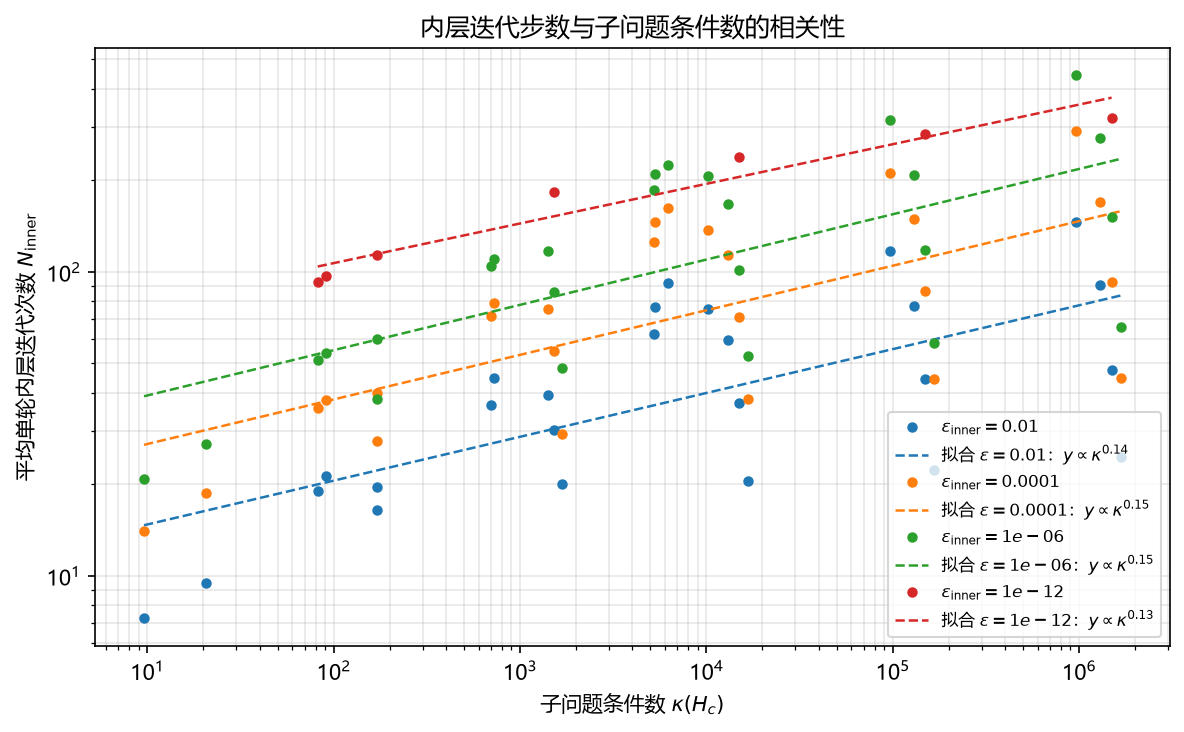
\includegraphics[width=0.8\textwidth]{figures/fig5_cond_corr.png}
\caption{内层迭代步数与子问题条件数的相关性（按内层精度分组拟合）}
\label{fig:cond-corr}
\end{figure}

结果显示：
\begin{itemize}
\item 在双对数坐标下，各组数据近似呈线性上升，支持内层迭代步数与 $\kappa(H_c)$ 之间存在幂律关系；
\item 四组拟合斜率均在 $0.13\sim0.15$ 之间，说明内层迭代步数对条件数的依赖较弱，与 CG 理论中 $\sqrt{\kappa}$ 的粗略上界相比，实际依赖更温和；
\item 内层精度越高（$\epsilon_{\mathrm{inner}}$ 越小），相同条件数下的迭代步数越多，曲线整体上移。
\end{itemize}

\subsection{研究假设检验总结}
\label{sec:res-summary}

综合上述结果，各研究假设的检验结论如下：

\begin{itemize}
\item \textbf{H1（支持）}：$c$ 增大总体提升外层收敛速率，同时增大单轮内层求解成本，二者形成权衡关系；
\item \textbf{H2（支持）}：不精确 ALM 场景下总计算代价随 $c$ 呈 U 型，存在内部最优 $c^*$；
\item \textbf{H3（部分支持）}：精确 ALM 场景下收敛平稳、无显著震荡；不精确 ALM 场景下大 $c$ 区域出现收敛平台/平稳性残差难以进一步下降。但“震荡”现象在本实验参数范围内并不普遍，因此只能说部分支持；
\item \textbf{H4（支持）}：内层精度越松，最优 $c^*$ 越小；
\item \textbf{H5（不支持，需修正）}：最优 $c^*$ 随 $\kappa(H)$ 增大并未如预期减小，反而略有增大。更准确的认识是：$c^*$ 不由 $\kappa(H)$ 单独决定，而由增广子问题条件数 $\kappa(H_c)$ 与外层收敛收益共同决定；$\kappa(H)$ 本身不是充分的参数选择指标。
\end{itemize}

\section{理论机制分析}
\label{sec:mechanism}

本节将实验结果与 ALM/CG 的理论性质联系起来，给出惩罚参数 $c$ 影响总计算代价的完整数学链条，并解释 H4、H5 的深层原因。

\subsection{外层加速：乘子误差传播}
\label{sec:mech-outer}

考虑精确 ALM 情形。设 $M_c=H+cA^\top A$，子问题精确解为 $x_{k+1}=M_c^{-1}(q-A^\top\lambda_k+cA^\top b)$。由 KKT 条件，最优乘子满足 $q=Hx^*+A^\top\lambda^*$ 和 $Ax^*=b$。记乘子误差 $e_{\lambda,k}=\lambda_k-\lambda^*$，经整理可得
\begin{equation}
\label{eq:multiplier-error}
e_{\lambda,k+1}=(I+cS)^{-1}e_{\lambda,k}, \qquad S=AH^{-1}A^\top\succ0.
\end{equation}
设 $S$ 的特征值为 $\mu_i>0$，则对应方向的收缩因子为
\begin{equation}
\label{eq:contraction}
\rho_i(c)=\frac{1}{1+c\mu_i}.
\end{equation}
因此 $c$ 越大，$\rho_i(c)$ 越小，外层乘子误差收敛越快。这解释了实验 1 中“$c$ 增大使原始残差下降更快”的现象。

\subsection{内层代价：CG 与子问题谱}
\label{sec:mech-inner}

内层用 CG 求解 $M_cx=rhs$。经典 CG 误差界给出达到精度 $\epsilon_{\mathrm{inner}}$ 所需迭代步数约为
\begin{equation}
\label{eq:mech-cg}
N_{\mathrm{CG}}\sim O\left(\sqrt{\kappa(M_c)}\,\log\frac1{\epsilon_{\mathrm{inner}}}\right).
\end{equation}
因此 $c$ 通过改变 $M_c=H+cA^\top A$ 的谱结构影响单轮内层成本。值得注意的是，由于 $A^\top A\succeq0$，$\lambda_{\max}(M_c)$ 与 $\lambda_{\min}(M_c)$ 都随 $c$ 单调不减，但 $\kappa(M_c)$ 是否上升取决于二者增长速率的相对大小；在本实验的大 $c$ 区域，$\kappa(M_c)$ 整体上升，导致 CG 成本增加。

\subsection{不精确 ALM 的平稳性误差地板}
\label{sec:mech-inexact}

若 CG 未精确求解，则存在内层残差 $\delta_k$ 使得
\begin{equation}
\label{eq:inner-residual}
M_cx_{k+1}=q-A^\top\lambda_k+cA^\top b+\delta_k.
\end{equation}
将乘子更新代入平稳性残差 $s_{k+1}=Hx_{k+1}-q+A^\top\lambda_{k+1}$，可得
\begin{equation}
\label{eq:stationarity-floor}
s_{k+1}=\delta_k.
\end{equation}
因此 $\|s_{k+1}\|=\|\delta_k\|$。当 CG 采用相对残差终止 $\|\delta_k\|\le\epsilon_{\mathrm{inner}}\|rhs_k\|$ 时，
\begin{equation}
\label{eq:error-floor}
\|s_{k+1}\|\lesssim\epsilon_{\mathrm{inner}}\|rhs_k\|.
\end{equation}
这意味着固定内层精度直接形成外层平稳性残差的误差地板：若 $\epsilon_{\mathrm{inner}}=10^{-4}$ 而外层要求 $\|s_k\|\le10^{-6}$，则无法保证达标。这从数学上解释了“除精确 ALM 外大量参数不满足终止条件”的初始现象\scite{fernandez2012}。

此外，不精确误差还会通过乘子更新进入外层迭代。设 $x_{k+1}=x_{k+1}^{\mathrm{exact}}+e_k$，$e_k=M_c^{-1}\delta_k$，则乘子更新中的扰动为 $cAM_c^{-1}\delta_k$。于是不精确 ALM 的乘子误差传播为
\begin{equation}
\label{eq:inexact-multiplier}
e_{\lambda,k+1}=(I+cS)^{-1}e_{\lambda,k}+cAM_c^{-1}\delta_k.
\end{equation}
前一项随 $c$ 增大而收缩（有利），后一项随 $c$ 增大而放大内层误差（不利）。这解释了大 $c$ 下不精确 ALM 更容易出现收敛平台的现象。

\subsection{总成本与 $c^*$ 的决定}
\label{sec:mech-ustar}

综合上述机制，总计算代价可近似表示为
\begin{equation}
\label{eq:total-cost}
C(c,\epsilon_{\mathrm{inner}})\approx N_{\mathrm{outer}}(c,\epsilon_{\mathrm{inner}})\cdot N_{\mathrm{CG}}(c,\epsilon_{\mathrm{inner}}),
\end{equation}
其中 $N_{\mathrm{outer}}$ 随 $c$ 增大而下降（来自收缩因子 $\rho(c)$），$N_{\mathrm{CG}}$ 随 $c$ 增大而上升（来自 $\kappa(M_c)$ 增大），二者竞争产生 U 型曲线与内部最优 $c^*$。

进一步，当 $\epsilon_{\mathrm{inner}}$ 减小时，$N_{\mathrm{CG}}$ 整体增大，减少一次外层迭代的边际收益变高，因此最优 $c^*$ 向右移动。这解释了 H4。

\subsection{H5 的深层原因：谱方向相互作用}
\label{sec:mech-h5}

H5 的原始假设 $\kappa(H)\uparrow\Rightarrow c^*\downarrow$ 隐含了“$\kappa(H)$ 能决定子问题难度”的假设。但外层收敛真正涉及 $S=AH^{-1}A^\top$，内层真正涉及 $H+cA^\top A$，二者都依赖于 $H$ 的特征向量方向与 $A$ 的约束方向之间的相对位置。设 $H=Q\Lambda Q^\top$，则
\begin{equation}
AH^{-1}A^\top=AQ\Lambda^{-1}Q^\top A^\top,
\end{equation}
其中 $AQ$ 明确刻画了这一相对位置；同理，$H+cA^\top A$ 的特征值并不是简单的 $\lambda_i(H)+c\lambda_i(A^\top A)$，除非 $H$ 与 $A^\top A$ 可同时对角化。因此，仅控制 $\kappa(H)$ 无法确定 $\kappa(H_c)$ 与外层收缩收益，H5 的因果链条少了一层。修正后的认识是：
\[
c^* \text{ 由 } \kappa(H_c) \text{（受 } H,\,A^\top A,\,c \text{ 谱结构共同决定）与外层收敛收益（受 } AH^{-1}A^\top \text{ 决定）共同决定。}
\]
这也解释了实验中不同 $\kappa(H)$ 的 $\kappa(H_c)$ 曲线发生交叉的现象。

\section{讨论与结论}
\label{sec:discussion}

本文围绕增广拉格朗日方法中的惩罚参数 $c$，通过“KKT reference + ALM + CG”的可复现实验体系，系统研究了 $c$ 对外层收敛行为、整体计算效率以及最优参数选择的影响。主要发现如下：

\begin{enumerate}
\item \textbf{外层收敛与内层成本存在 U 型权衡}：$c$ 增大加快原始残差收敛，但同时提高子问题条件数 $\kappa(H_c)$ 与单轮内层求解成本，因此总计算代价随 $c$ 呈 U 型，存在计算最优 $c^*$。
\item \textbf{内层精度改变成本权衡的相对重要性}：$\epsilon_{\mathrm{inner}}$ 越严，单次内层求解越昂贵，减少外层迭代的边际收益越大，导致 $c^*$ 向较大区域移动。这为 H4 提供了机制层面的解释，而不仅是现象描述。
\item \textbf{$\kappa(H)$ 不是预测 $c^*$ 的充分指标}：实验表明 $c^*$ 随 $\kappa(H)$ 增大略微增大，与 H5 的初始预期相反。进一步分析显示，真正决定内层求解难度的量是增广子问题条件数 $\kappa(H_c)$，而 $\kappa(H_c)$ 同时受 $c$、$A^\top A$ 以及二者谱结构相互作用的影响。因此，H5 应修正为：$c^*$ 由增广后子问题的谱性质与外层收敛收益共同决定。
\end{enumerate}

本文的结论可以概括为：惩罚参数 $c$ 并不是一个可以脱离问题结构而固定的 ALM 常数；其最优取值依赖于内层求解精度以及增广后子问题的实际数值条件。这一认识对于实际使用 ALM 时进行参数自适应具有直接指导意义。

本研究的局限性包括：参数网格较粗（$c$ 按数量级扫描），$c^*$ 的精确位置可能位于网格之间；实验仅覆盖对称正定二次规划基准问题；自适应 $c$ 策略（实验 4）尚未纳入本文结果。后续工作可以在 $c^*$ 附近加密网格，并进一步验证自适应策略在问题特性未知时的表现。

\begin{thebibliography}{9}

\bibitem{bertsekas1982}
D.~P. Bertsekas.
\emph{Constrained Optimization and Lagrange Multiplier Methods}.
Academic Press, 1982.

\bibitem{hestenes1952}
M.~R. Hestenes and E.~Stiefel.
Methods of conjugate gradients for solving linear systems.
\emph{Journal of Research of the National Bureau of Standards}, 49(6):409--436, 1952.

\bibitem{fernandez2012}
D.~Fern\'andez and M.~V.~Solodov.
Local convergence of exact and inexact augmented Lagrangian methods under the second-order sufficient optimality condition.
\emph{SIAM Journal on Optimization}, 22(2):384--407, 2012.

\end{thebibliography}

\end{document}